\subsection{Passage throughflow} \label{sec:throughflow}
As discussed in \cref{sec:throughflowp} the passage throughflow is calculated by using the BSF. To do this a suitable location was chosen for each time step and passage such that there are no boundaries next to the passageways. This method is the same for each of the passages, noting that only zonal flow was studied. Thus we can study the effect of changes in bathymetry on the relative strength of the flow.  The studied passageways are labeled in \cref{fig:passages_ocean}. The computed throughflow can be seen in \cref{fig:throughflow}. The onset of the ACC is visible. With the onset of the ACC a reversal of flow between the Indian and Pacific oceans is seen. Showing that due to the northward movement of Australia and the deepening of the drake passage the total volume transported by the ACC grows dramatically over time. Furthermore, it can be seen that the opening of the drake passage causes the flow through the Aghulas passage to reverse in direction. Also, the throughflow through the Panama passage is shown to slow due to both the onset of the ACC and the closure of the Tethys Seaway. Finally the direction of flow through the Panama passage is reversed after 15Ma due to the total closure of the Tethys Seaway. The reversal of the Indonesian throughflow observed by \cite{Mulder2017Jul} is not observed with total throughflow always moving water east to west. This is however in agreement with the flow found by \cite{omta2003physical} in a shallow-water model. Note, however, that the bathymetries used by their paper deviate dramatically from the ones used here.


To get a better understanding of the flows, we look at a vector field showing the direction of horizontal water displacement for each of the timesteps. This is done by making a weighted mean of the horizontal flow field for each layer weighted by the volume of each grid cell. Each vector represents the total flow for each full depth grid cell. Thus showing the total velocity field of the ocean and the subsequent direction of water displacement. The velocity fields are plotted in  \cref{fig:flowfield}. Here the ACC is again very noticeable. The reversal of flow through the Panama passage at $15Ma$ is the most interesting result here.  Where here we find the closure of the Thetys seaway to be the main factor. However, the reversal only occurs after the closure of the seaway. This result is similar to what was found by \cite{omta2003physical} where the flow reversal was also observed to coincide with the closure of the Thetys Seaway.

The largest changes in the velocity field are observed in the Indian Ocean. The Indian continent moves northward at a very fast pace. After 55 Ma the flow through the passage north of the Indian continent is massively reduced and instead, the water flows east of the continent into the Tethys Seaway. No current circulating India is observed in any of the time steps. The position of the Indian continent does however seem to have a strong influence on the strength of the Aghulas sub-tropical gyre. This can probably be explained by the amount of water that is transported through the Tethys seaway. A closer inspection of this gyre can be found in \cref{sec:BSF}.

\begin{figure}[H]
	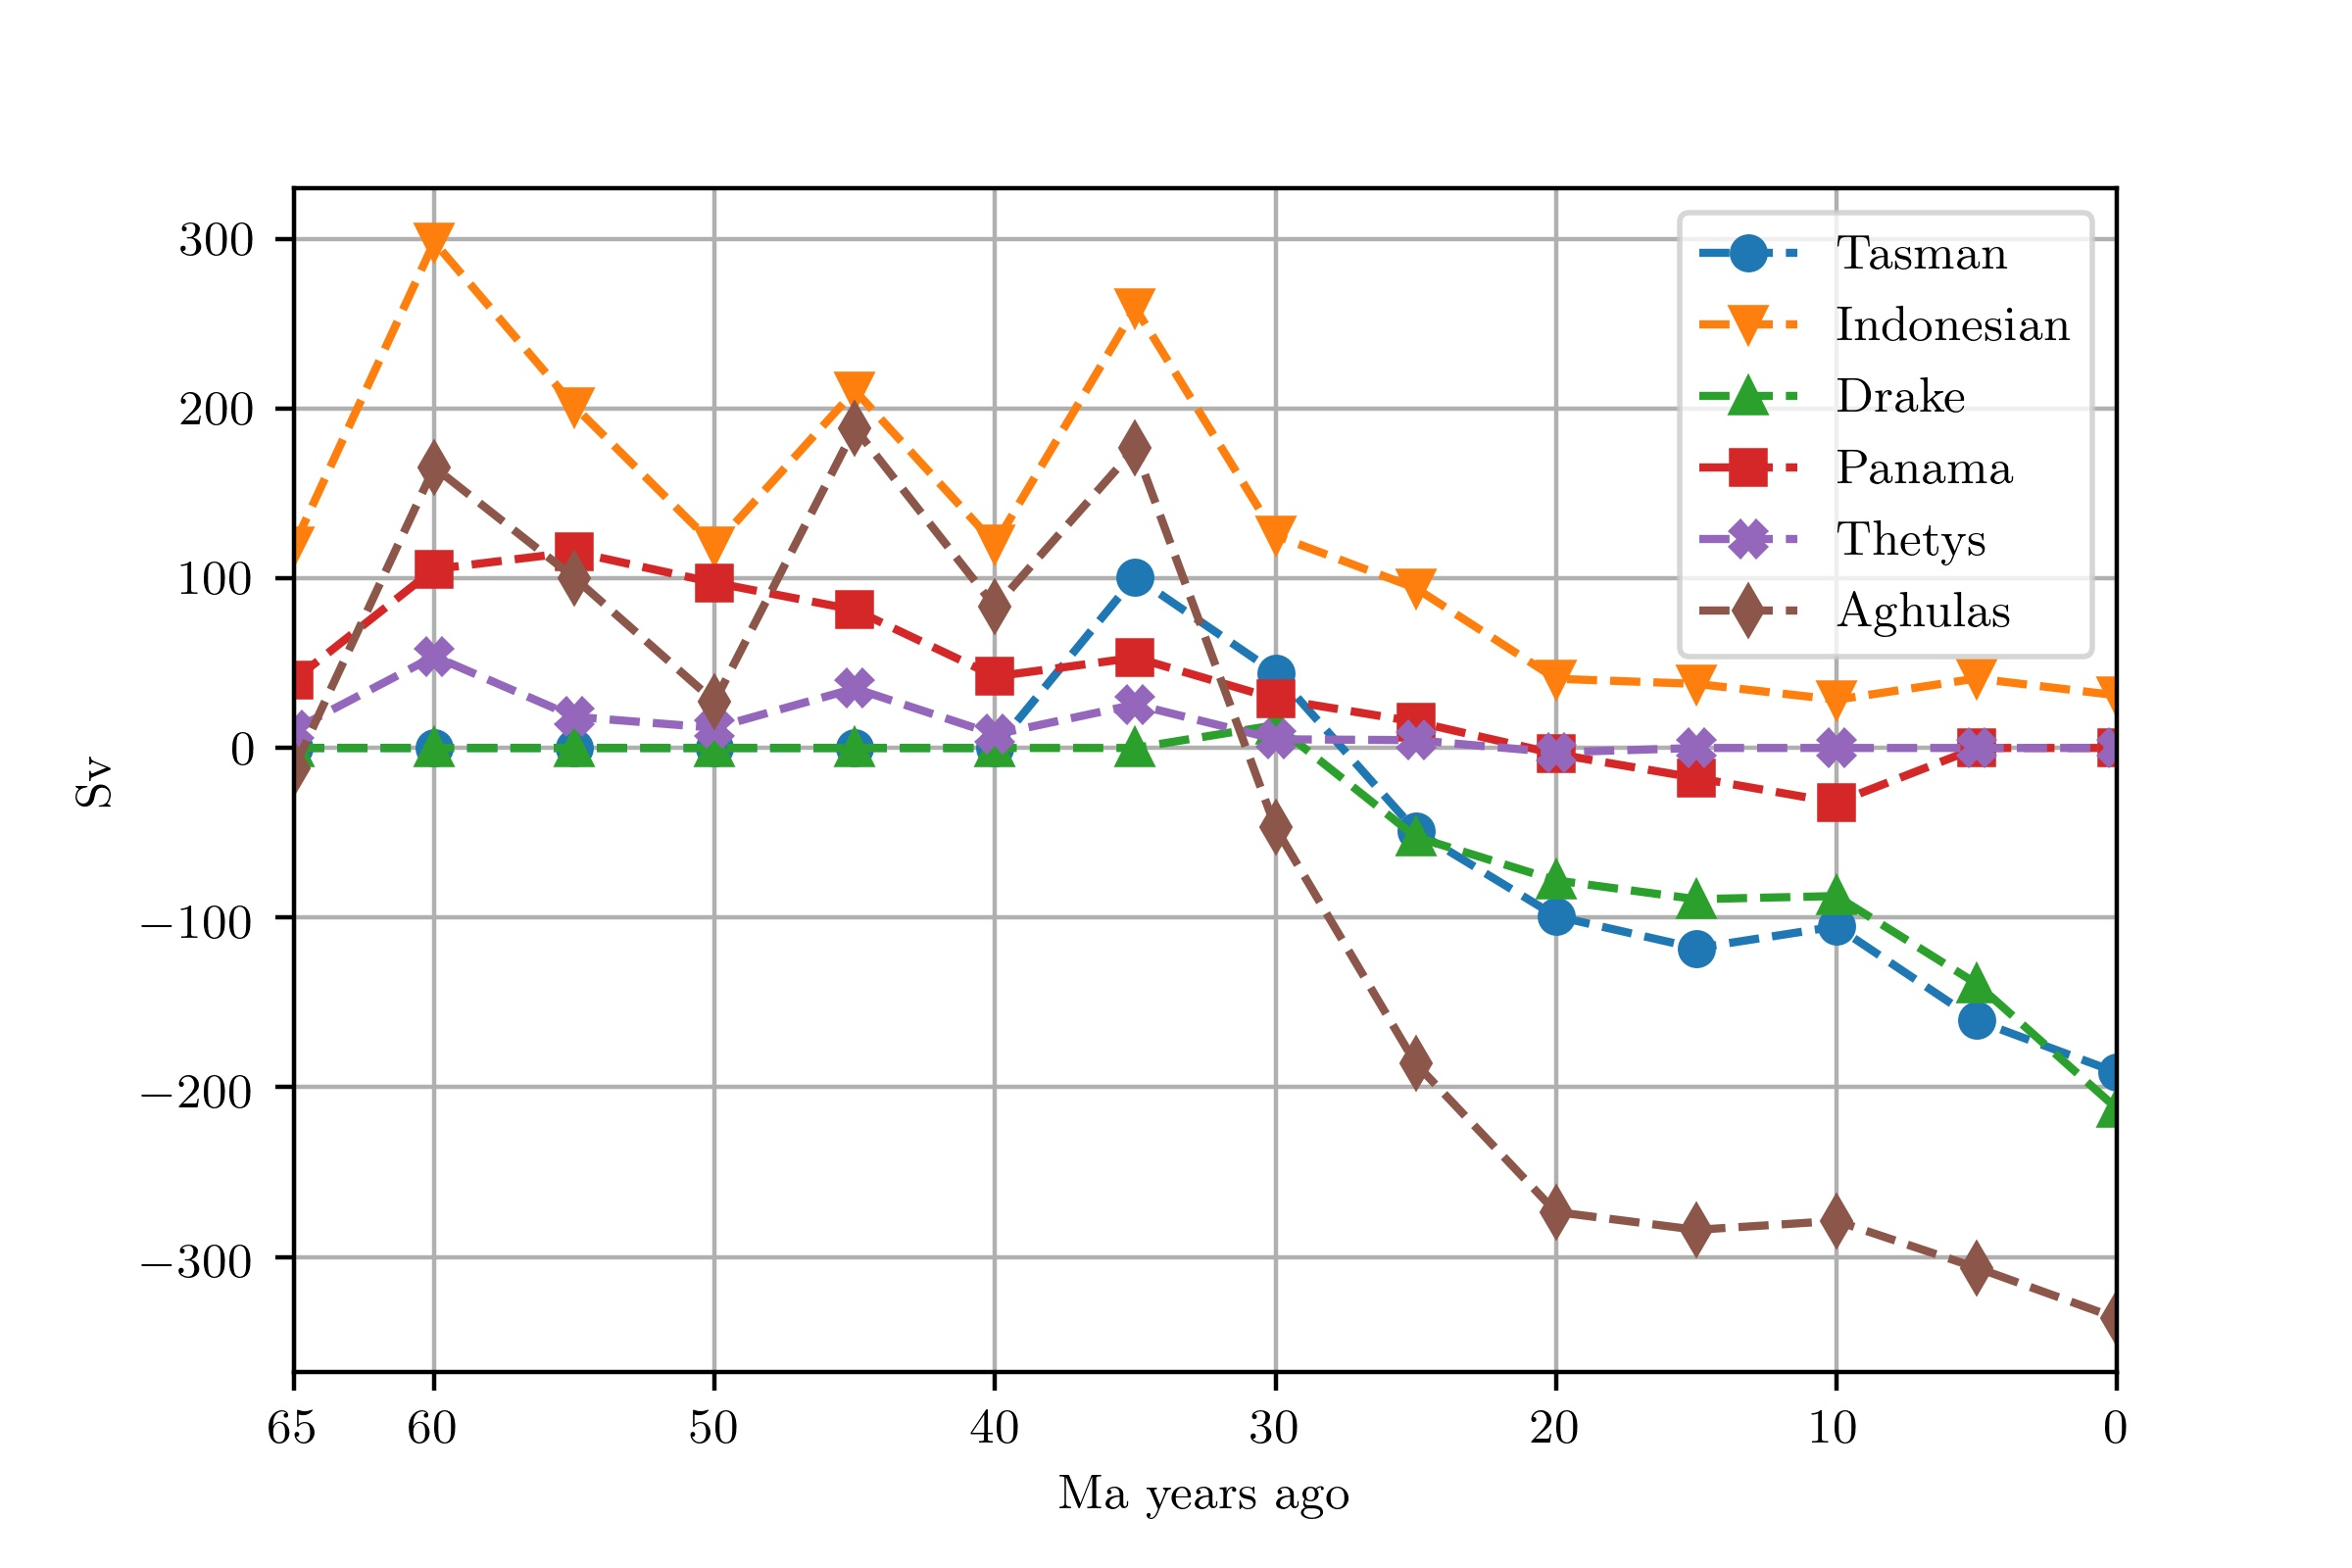
\includegraphics[width=\linewidth]{throughflow_bsf}
	\caption{Total volume transport in Sverdups for 7 passages. Running from 65 milion years ago to the present day situation. Positive values indicate transport to the west}
	\label{fig:throughflow}
\end{figure}
%TODO maybe something on nothern subpolar gyre?